\documentclass[output=paper,colorlinks=true,citecolor=brown]{langscibook}
%\documentclass{article}
% ,hidelinks
% showindex]

\author{András Kornai\orcid{0000-0001-6078-6840}\affiliation{Budapest University of Technology and Economics}}


\IfFileExists{../localcommands.tex}{
   \addbibresource{../localbibliography.bib}
   \usepackage{orcidlink}
\usepackage{tabularx,multicol}
\usepackage{url}
\urlstyle{same}

\usepackage{siunitx}
\sisetup{group-digits = none}

\usepackage{langsci-branding} 
\usepackage{langsci-optional}
\usepackage{langsci-lgr}
\usepackage{langsci-tbls}
\usepackage{langsci-gb4e}

% Müller
\usepackage{tikz-qtree}
\usepackage{hologo}

% 3_pullum.tex
\usepackage{langsci-textipa}

% 8_levine
\usepackage{bm}
\usepackage{umoline}
\usepackage{pifont}
\usepackage{pstricks,pst-node,pst-tree}
\usepackage{ulem}
\usepackage{mathrsfs}
\usepackage{bussproofs}

% 14_kornai
\usepackage[matrix,arrow]{xy}
\usepackage{subcaption}

\usepackage[linguistics, edges]{forest}
\usetikzlibrary{arrows, arrows.meta}

   \SetupAffiliations{output in groups = false,
                   orcid placement = after,
                   separator between two = {\bigskip\\},
                   separator between multiple = {\bigskip\\},
                   separator between final two = {\bigskip\\}
                   }

% ORCIDs in langsci-affiliations 
\definecolor{orcidlogocol}{cmyk}{0,0,0,1}
\RenewDocumentCommand{\LinkToORCIDinAffiliations}{ +m }
  {%
    \,\orcidlink{#1}%
  }

\makeatletter
\let\thetitle\@title
\let\theauthor\@author
\makeatother

% Cite and cross-reference other chapters
\newcommand{\crossrefchaptert}[2][]{\citet*[#1]{chapters/#2}, Chapter~\ref{chap-#2} of this volume} 
\newcommand{\crossrefchapterp}[2][]{(\citealp*[#1]{chapters/#2}, Chapter~\ref{chap-#2} of this volume)}
\newcommand{\crossrefchapteralt}[2][]{\citealt*[#1]{chapters/#2}, Chapter~\ref{chap-#2} of this volume}
\newcommand{\crossrefchapteralp}[2][]{\citealp*[#1]{chapters/#2}, Chapter~\ref{chap-#2} of this volume}

\newcommand{\crossrefcitet}[2][]{\citet*[#1]{chapters/#2}} 
\newcommand{\crossrefcitep}[2][]{\citep*[#1]{chapters/#2}}
\newcommand{\crossrefcitealt}[2][]{\citealt*[#1]{chapters/#2}}
\newcommand{\crossrefcitealp}[2][]{\citealp*[#1]{chapters/#2}}


\newcommand{\sub}[1]{\textsubscript{\scriptsize\textrm{#1}}}
% Müller
\newcommand{\page}{}

\let\citew\citet
\def\underRevision{Revise and resubmit}
\let\textbfemph\emph

%% % taken from https://tex.stackexchange.com/a/95079/18561
\newbox\usefulbox

\makeatletter
\def\getslant #1{\strip@pt\fontdimen1 #1}

\def\skoverline #1{\mathchoice
 {{\setbox\usefulbox=\hbox{$\m@th\displaystyle #1$}%
    \dimen@ \getslant\the\textfont\symletters \ht\usefulbox
    \divide\dimen@ \tw@ 
    \kern\dimen@ 
    \overline{\kern-\dimen@ \box\usefulbox\kern\dimen@ }\kern-\dimen@ }}
 {{\setbox\usefulbox=\hbox{$\m@th\textstyle #1$}%
    \dimen@ \getslant\the\textfont\symletters \ht\usefulbox
    \divide\dimen@ \tw@ 
    \kern\dimen@ 
    \overline{\kern-\dimen@ \box\usefulbox\kern\dimen@ }\kern-\dimen@ }}
 {{\setbox\usefulbox=\hbox{$\m@th\scriptstyle #1$}%
    \dimen@ \getslant\the\scriptfont\symletters \ht\usefulbox
    \divide\dimen@ \tw@ 
    \kern\dimen@ 
    \overline{\kern-\dimen@ \box\usefulbox\kern\dimen@ }\kern-\dimen@ }}
 {{\setbox\usefulbox=\hbox{$\m@th\scriptscriptstyle #1$}%
    \dimen@ \getslant\the\scriptscriptfont\symletters \ht\usefulbox
    \divide\dimen@ \tw@ 
    \kern\dimen@ 
    \overline{\kern-\dimen@ \box\usefulbox\kern\dimen@ }\kern-\dimen@ }}%
 {}}
\makeatother

% 1_intro.tex

% For the block quote:
\definecolor{linequote}{RGB}{224,215,188}
\definecolor{backquote}{RGB}{249,245,233}

\NewDocumentEnvironment{myquote}{ +m }
  {%
    \begin{tblsfilled}{}[black!12]
    #1%
  }
  {\end{tblsfilled}}

% 2_gibson.tex


% Example(s) Environments
% 12pt, No new-lines after example number is printed

\newcounter{examplectr}
\newcounter{fnexamplectr}

% Note: don't use subexamples in footnotes.

% This line is to overcome a bug in cmu-art style: it prints counter
% values to the aux file using \theaux... rather than using \the...
\def\theauxexamplectr{\theexamplectr}

\newcounter{subexamplectr}
\def\theauxsubexamplectr{\thesubexamplectr}
\def\theauxfnexamplectr{\thefnexamplectr}

\renewcommand{\theexamplectr}{\arabic{examplectr}}
% This command causes example numbers to appear without following periods

\renewcommand{\thefnexamplectr}{\roman{fnexamplectr}}
% This command causes example numbers to appear without following periods

\renewcommand{\thesubexamplectr}{\theexamplectr\alph{subexamplectr}}
% This command gives the number of an example and subexample as e.g. 1a, 2b

\newlength{\wdth}
\newcommand{\strike}[1]{\settowidth{\wdth}{#1}\rlap{\rule[.5ex]{\wdth}{1pt}}#1}

\newcommand{\exref}[1]{(\ref{#1})}
% This command puts reference numbers with parentheses
% surrounding them 

% The environment ``examples'' gives a list of examples, one on each line,
% numbered with a lower case alphabetic character
\newenvironment{examples}%
   { \vspace{-\baselineskip}
     \begin{list}%
     \textrm{\alph{subexamplectr}.}%
     {\usecounter{subexamplectr}
     \setlength{\topsep}{-\parskip}
     \setlength{\itemsep}{-2pt}
     \setlength{\leftmargin}{0.5in}
     \setlength{\rightmargin}{0in} } }%
   { \end{list}}

% The environment ``myexample'' outputs an arabic counter ``examplectr''
% surrounded by parentheses.
\newenvironment{myexample}
   { \vspace{20pt}
     \noindent
     \begin{minipage}{\textwidth}    % minipage environment disallows
                 % breaks across pages

     \refstepcounter{examplectr}     % step the counter and cause this
                 % section to be referenced by the
                 % counter ``examplectr''
     (\arabic{examplectr})}%
   { \vspace{20pt}
     \end{minipage}}

\newenvironment{myfnexample}
   { \vspace{2pt}
     \noindent
     \begin{minipage}{\textwidth}    % minipage environment disallows
                 % breaks across pages

     \refstepcounter{fnexamplectr}     % step the counter and cause this
                 % section to be referenced by the
                 % counter ``examplectr''
     (\roman{fnexamplectr})}%
   { \vspace{2pt}c
     \end{minipage}}
    
\newcommand*\circled[1]{\tikz[baseline=(char.base)]{
            \node[shape=circle,draw,inner sep=2pt] (char) {#1};}}

\newcommand{\data}[1]{\textit{#1}}
\newcommand{\nodata}[1]{#1}
\newcommand{\blank}{\rule{1.2em}{0.5pt}}
\newcommand{\pt}[1]{\ensuremath{\mathsf{#1}}}
\newcommand{\ptv}[1]{\ensuremath{\textsf{\textsl{#1}}}}
\newcommand{\sv}[1]{\ensuremath{\mathcal{#1}}}

\newcommand{\sX}{\sv{X}}
\newcommand{\sF}{\sv{F}}
\newcommand{\sG}{\sv{G}}
\newcommand{\greekp}{\upvarphi}
\newcommand{\greekr}{\uprho}
\newcommand{\greeks}{\upsigma}
\newcommand{\MultiLine}[1]{\ensuremath{\begin{array}[b]{@{}l@{}}#1\end{array}}}
\newcommand{\LexEnt}[3]{#1; \ensuremath{#2}; \syncat{#3}}

\newcommand{\LexEntBroken}[3]
  {\Shortstack
      {%
        {#1;} 
        {\ensuremath{#2};} 
        {\syncat{#3}}%
      }%
  }

\newcommand{\grey}[1]{\colorbox{mycolor}{#1}}
\definecolor{mycolor}{gray}{0.8}

\newcommand{\gap}{\longrule}
\newcommand{\gp}{\gap}
\newcommand{\vs}{\raisebox{.05em}{\ensuremath{\,\upharpoonright}}}

\newcommand{\E}{ε}

\newcommand{\EBob}[1]{\textsl{#1}}

\newcommand{\B}{\textbf}
\newcommand{\f}{{\color{green}f}}  % Question what does f do? It does not have any output in the
                                % original PDF
%\newcommand{\Lemma}{{\color{pink}Lemma}}
\newcommand{\Lemma}{\ensuremath{\vdots\hskip.5cm\vdots}\noLine}

%\newcommand{\calP}{{\color{pink}calP}} % Sebastian
\newcommand{\calP}{\ensuremath{\mathcal{P}}}


\newcommand{\maru}[1]{\ooalign{\hfil#1\/\hfil\crcr
      \raise.05ex\hbox{\LARGE\mathhexbox20D}}}


%\newcommand{\sem}[2][M\!,g]{\mbox{$[\![ \mathrm{#2} ]\!]^{#1}$}}
\newcommand{\sem}{\ensuremath}

%
\newcommand{\trns}[1]{\textbf{#1}\xspace}
\newcommand{\bs}{{\textbackslash}}
\newcommand{\bsl}{{\bs}}
\newcommand{\fb}[1]{\textsubscript{#1}}
\newcommand{\syncat}[1]{\ensuremath{\mathrm{#1}}}
\newcommand{\term}[1]{\textit{#1}}
\newcommand{\LemmaAlt}{\ensuremath{\vdots\hskip.5cm\vdots}}
\NewDocumentCommand{\VanLabel}{m}{\MakeUppercase{#1}}

   %% hyphenation points for line breaks
%% Normally, automatic hyphenation in LaTeX is very good
%% If a word is mis-hyphenated, add it to this file
%%
%% add information to TeX file before \begin{document} with:
%% %% hyphenation points for line breaks
%% Normally, automatic hyphenation in LaTeX is very good
%% If a word is mis-hyphenated, add it to this file
%%
%% add information to TeX file before \begin{document} with:
%% %% hyphenation points for line breaks
%% Normally, automatic hyphenation in LaTeX is very good
%% If a word is mis-hyphenated, add it to this file
%%
%% add information to TeX file before \begin{document} with:
%% \include{localhyphenation}
\hyphenation{
    Ber-ti-net-to
    caus-a-tive
    fest-schrift
    Fest-schrift
    Hix-kar-ya-na
    In-do-ne-sian
    mor-pho-phon-o-log-i-cal
    Mo-se-tén
    par-a-digm
    phra-ses
    Que-chua
}

\hyphenation{
    Ber-ti-net-to
    caus-a-tive
    fest-schrift
    Fest-schrift
    Hix-kar-ya-na
    In-do-ne-sian
    mor-pho-phon-o-log-i-cal
    Mo-se-tén
    par-a-digm
    phra-ses
    Que-chua
}

\hyphenation{
    Ber-ti-net-to
    caus-a-tive
    fest-schrift
    Fest-schrift
    Hix-kar-ya-na
    In-do-ne-sian
    mor-pho-phon-o-log-i-cal
    Mo-se-tén
    par-a-digm
    phra-ses
    Que-chua
}

   \boolfalse{bookcompile}
   \togglepaper[23]%%chapternumber
}{}


\title{What is the simplest semantics imaginable?}




\abstract{We claim
that three binary relations, 0, 1, and 2, are both necessary and sufficient
for formal semantics: 1 and 2 are the well-known ``subject of'' and ``object of''
relations, and 0 corresponds to the subsumption or ``is a'' relationship well
known from knowledge representation. We describe how these can be used to
compositionally assign a semantic representation built from primitives
(morphemes, semantic atoms) and how the system can be related to the
computational ``word vector'' semantics which is surprisingly effective even
though it appears to employ no grammatical rules or constraints.}

\begin{document}
\maketitle

%move the following commands to the "local \ldots " files of the master project when integrating this chapter
\section{Introduction}

There is no evidence that in English the vestigial system of object marking can
be extended beyond personal pronouns, yet we have little doubt that English
speakers can fully grasp transitive constructions involving inanimate
objects. Since most linguists assume that coordination and subordination will
be present in every language, Everett's discovery of a language lacking
syntactic facilities for these is seen as some grave error akin to a
hypothetical discovery of a language lacking subjects and objects. But when
viewed from the perspective of semantics, impoverished syntax is no more
surprising than impoverished morphology, so the question should be: what is
the absolute minimum we require for semantics?

In this paper, we start from the simplest imaginable cases, subject-predicate
and modifier-head constructions, and gradually build up a system of semantic
representation both in the tradition of Knowledge Representation (KR; 
\cite{Brachman:2004}) and in the contemporary ``thought vector'' approach
\citep{LeCun:2015,Kornai:2022}. These are not competing but complementary
views of the same subject matter, both true at the same time like the
algebraic and the function-theoretic views of polynomials. While the KR view
does not significantly depart from the common linguistic view that
structures are to be represented by some kind of graphs (an idea common to
transformational and dependency grammar formalisms), the vector approach is
very unfamiliar: if the representations are $n$-tuples of numbers, what are
the rules?

This question is especially vexing in light of the observation that the main
vector operation, vector addition, plays only a marginal role in the
computational system: it is used for solving analogical puzzles like \textit{France is to Germany as Paris is to X} \citep{Mikolov:2013l} and little
besides. Using the KR side to explore the issue we find that three binary
operations, 0, 1, and 2, are both necessary and sufficient for formal
semantics. 1 and 2 are the well-known ``subject of'' and ``object of''
relations, and 0 corresponds to the subsumption relationship known as ``is a''
in KR and as hyponymy in lexicography. (The vector equivalents of these
operations are somewhat more technical, and are not required for making our
main point that the minimum is three -- see \citet{Kornai:2022} for details.)

The sufficiency of these operations is not trivial -- students of Relational
Grammar and many similar systems will no doubt wonder about ``3'' and perhaps
different kinds of linkers such as thematic (proto)roles or k\={a}rakas. For
indirect objects, the reader is referred to \citet{Kornai:2012}, and for deep
cases, thematic roles and k\={a}rakas see Chapter 2.4 of \citet{Kornai:2022}.
The main line of attack in reduction to ``1'' and ``2'' is that ``3'' can itself be
considered (together with other conceptual relations typically expressed by
case markers and adpositions) to have their own subjects and (prepositional)
objects. This will of course complicate the graphs (in ways that will be
familiar from generative semantics) but ensure that we will never need
hyper\textit{edges} just hyper\textit{nodes}. The resulting system is rather similar
to the
\href{https://en.wikipedia.org/wiki/Resource_Description_Framework}{Resource
  Description Framework} used in the
\href{https://en.wikipedia.org/wiki/Semantic_Web}{Semantic Web} where binary
relations are encoded in a (subject verb object) triple. Since such
triples can be substituted for one another, for \textit{give} we obtain an analysis
``cause to have'' so that \textit{x gives y to z} becomes \texttt{(x cause (z has
  y))}. This method is immune to the standard criticisms \citep{Fodor:1970}
leveled against generative semantics-style meaning decomposition that were
based on the pronominalization possibilities of the `to + inf' natural
language paraphrase, since the formulas explicitly contain this information.
\citet{Kornai:2010} discusses how the other criticism, that such a
decomposition (cause to die $\rightarrow$ cause not to have life functions
$\rightarrow$ cause not to metabolize, respond, \ldots) may never terminate,
is actually irrelevant in an algebraic setup that enables circularity, and
\citet{Kornai:2012} describes how higher arity verbs, such as \textit{promise} can
be handled in the same manner. 

But the necessity of three different operations is even less trivial: after all,
natural language semantics is often viewed as translation to First Order
Predicate Calculus (FOPC; \cite{Blackburn:2015}) and via combinators
\citep{Curry:1958} FOPC can be reduced to strings of a single symbol $J$ with
the appropriate parenthetization (\cite{Schoenfinkel:1924}, English
transl. \cite{Heijenoort:1967}). We can take the no-frills approach further,
since the parens can be eliminated in favor of Reverse Polish Notation (RPN),
leaving us with binary strings. As the first symbol is always $J$, which we
denote by `1', we can use `0' for the binary operator symbol of RPN, and we
are guaranteed that each well-formed predicate formula corresponds to a unique
integer written in base 2. Furthermore, the translation between the original
formula and the binary number is computable mechanistically in either
direction by a rather simple Turing machine. Taking this to the extreme,
binary integers can be written in base 1, and again translation between the
formats by a Turing machine is available in both directions, so that all we need
is a single symbol which can be repeated as many times as we need. If we are
happy with integers, base unspecified, Gödel numbering would work just as
well.

This is not just a walk through some rarely visited pages of the mathematical
logic bestiary. There are sophisticated attempts at using combinatory logic in
semantics since the 1980s \citep{Szabolcsi:1987,Steedman:1987,Jacobson:1999,Baldridge:2002}, with
important links to mild context sensitivity\slash polynomial parsability
\citep{Joshi:1990}. Clearly, neither FOPC nor higher order intensional calculi
such as those employed in Montague Grammar have a privileged status as the One True
Formalism (OTF) for semantics, and the search for OTF is not a trivial one. Our
argument will rely on a stricter understanding of compositionality than the
one generally assumed: while the mapping from Gödel numbers (or binary
strings) back to logic formulas is unique, and Turing-computable, not every
such mapping is compositional in the accepted sense of taking some string X,
decomposing it \textit{by simple means} as AB, and computing the meaning of
the whole from the meanings of the parts A and B. 

In \sectref{expect} we set expectations by discussing some important
desiderata for OTF.  We also introduce some less commonly taught desiderata
students of linguistic semantics may not even have heard of, such as \textit{smooth transition from morphology to syntax} and \textit{embeddability}, and
argue that these are actually part of the same cluster of desiderata.  Our own
proposal, the \texttt{4lang} system (see \url{https://github.com/kornai/4lang/tree/master/V2}), is discussed in
\sectref{4lang}, where we return to the issue whether there is, or should
be, a minimal system among the proposals meeting the desiderata.

\section{What do we expect of semantics?}\label{expect}

Let us begin with some standard desiderata: 

\begin{enumerate}
\item[D1] Comes with reasonable model theory
\item[D2] Reasonably simple (compositional) mapping from natural language to
  OTF
\item[D3] Mapping in the reverse direction into passable natural language so that
  OTF can serve as a translation pivot
\item[D4] Usable for disambiguation
\item[D5] Usable for characterizing synonymy
\item[D6] Extends smoothly to verbal description of non-verbal material (music,
  scientific models, functional description of algorithms, \ldots)
\end{enumerate}


\noindent
D1 is taken very seriously by proponents of logical
semantics, who treat all other approaches (by natural language paraphrase, by
diagrams, and by KR in general) as \textit{markerese} since \citet{Lewis:1970}.
To satisfy this, OTF must contain three well-defined parts: a language of
formulas $L$, a collection of models $\mathcal{M}$, and an interpretation
relation $i: L \rightarrow \mathcal{M} $ between the two \citep{Tarski:1956}.
By well-defined we mean the existence of effective procedures to decide 
whether something is a (well-formed) formula and to decide whether something
amounts to a model. The mapping itself needs to be not just effective (Turing-computable), but computable in a particularly simple manner we will discuss at
D8 below. 

For linguistic semantics to follow the same architecture one would expect $L$
to contain all well-formed (grammatical) strings, and only these, and would
use $\mathcal{M}$, the collection of models, to capture the world that is
being talked about, with $i$ mapping elements of the language onto their
meanings.  In reality, Montague Grammar (MG; \cite{Montague:1970,Montague:1973}) represents a
considerable departure from this architecture. On the left side, we do not
find $L$, natural language, but $D$, \textit{disambiguated language}, a
theoretical construct that contains not just the well-formed expressions of
language but also their constituents and derivation histories (see discussion
of D4 below).

\begin{figure}[h]
% % \centering
% % \mbox{\xymatrix{
% % L \ar[r]^d &D\ar[r]^t &F\ar[r]^I & \mathcal{M}\ar[r]^g &W\\
% % }}
\begin{tikzpicture}[>={Stealth[round]}]
    \node (L) at (0,0) {$L$};
    \node (D) at (2,0) {$D$};
    \node (F) at (4,0) {$F$};
    \node (M) at (6,0) {$\mathcal{M}$};
    \node (W) at (8,0) {$W$};
    
    \draw[->] (L) -- (D) node [midway,above] {$d$};
    \draw[->] (D) -- (F) node [midway,above] {$t$};
    \draw[->] (F) -- (M) node [midway,above] {$I$};
    \draw[->] (M) -- (W) node [midway,above] {$g$};
\end{tikzpicture}
\caption{Information objects associated with MG}
\label{fig:information_objects}
\end{figure}

On the right side, we do not find real-world objects or even formal objects
(models), but formulas $F$ of a particular logic calculus. The full picture of
MG is composed of the first two or three arrows in
\figref{fig:information_objects}, with the primary attention focused on the
translation homomorphism $t$. The models $\mathcal{M}$ are reasonably standard
set-theoretical constructs (except for an internal time parameter that
temporal semantics often relies on), and the grounding $g$ in the real world
is completely left out -- Montague was no doubt familiar with Quine's and
others' criticism of direct reference.

The disambiguation mapping $d$ is an elegant technical device that helps a
great deal in simplifying subsequent stages of the mapping. Unfortunately,
scholars in the MG tradition have spent little effort on building grammatical
models of natural language that could serve as a starting point for
disambiguation in the sense Montague urged, and the use of $d$ in semantics is
more a promissory note than an actual algorithmic method. In this key respect,
MG actually fails D4.

D2 is also taken very seriously, so much so that important
ranges of phenomena where it obviously fails, such as noun-noun compounding,
are simply declared out of scope for semantics. \citet{Fodor:1998} is typical
in treating all word meanings as atomic, i.e. ignoring all productive
morphological phenomena. This of course requires the memorization of all word
meanings and brings back the psychological problem
\citep{Partee:1979,Partee:2013} of accounting for infinite data sets in a
finite brain.

Clearly, expressions like \textit{ropeladder} `ladder made of rope,' \textit{testtube} `tube used for testing,' and \textit{manslaughter} `slaughter undergone
by man' \citep{Kiparsky:1982b} are not entirely compositional. Equally
clearly, the meaning of novel compounds is largely predictable, as are the
meanings conferred by productive derivational processes. The Lexicalist
Hypothesis \citep{Chomsky:1970} segregating morphology from syntax is clearly
untenable \citep{Bruening:2018}, and in its place we offer our own
desideratum:

\begin{itemize}
\sloppy 
\item[D7] 
  Compositional (syntactic) and non-compositional (morphological)
  processes must be part of the same continuum
\end{itemize}

In other words, there cannot be a different semantics for morphology and for
syntax, especially as the border between the two is not uniform across
languages. It must be one and the same interpretation mechanism that takes you
``from morpheme to utterance''. This is not to say that there is no \textit{word}
unit that syntax can refer to (the classical psycholinguistic evidence in
favor of memorized units with lexicalized meanings cited in \citet{Muller:2018}
is hardly controvertible), but simply to insist on deriving as much of this
meaning by compositional means as possible. In \sectref{4lang} we offer a
mechanism that deals with the non-compositional aspects by means of subdirect
products, which contain the fully compositional direct products as a limiting
case.

D3, while in principle compatible with many theories, is
seriously underresearched. Using a natural language (typically English) as
pivot (intermediary) between two languages is common both in manual and in
machine translation. The use of a formal language is almost unheard of: the
only proposal with actual translations is Universal Networking Language
\citep{Cardenosa:2005}, and the use of logic formulas is unattested. Given how
common it is to consider semantics ``the language of thought,'' the
single-minded focus on translation to, but never from, mentalese is rather
surprising.

This onesidedness cannot be entirely attributed to the fact that systems of
translation to logic formulas (including descendants of MG such as Dynamic
Predicate Logic) have very little coverage to begin with. It appears the real
issue is lack of transparency, a phenomenon well observable on the
Schönfinkel-style reduction step of replacing the standard $S$ and $K$ 
combinators by a single combinator $J$. This  $J$ is defined by cases:
\[
  Jx =
  \begin{cases}
%    U & \text{if } x=C\\
    K & \text{if } x=S\\
    S & \text{otherwise}
  \end{cases}
\]

\noindent
Therefore, we have $JJ = S; J(JJ)= JS = K$ eliminating the original $S$ and $K$
entirely in favor of a single entity. Notice that the method would be just as
applicable if we didn't have 2 things to reduce but 52. We would only need to
stretch the case-by-case definition accordingly (see \cite[Chapter 1E4]{Curry:1958}). 

For a concrete example, consider the translation of the English reflexive
pronoun \textit{himself} which \citet{Szabolcsi:1987} argues to be the combinator
$W$, defined as $W x y = x y y$. In the standard $S,K$ basis $W$ is
expressible as $((SS)(SK))$ so $W$ is $(((JJ)(JJ))((JJ)(J(JJ))))$. Continuing
with the no-frills approach, the order of applications encoded in the
parenthetization can be just as well encoded by RPN, using the operator symbol
$\circ$. This will make the formula into $JJ\circ JJ\circ \circ
JJ\circ J JJ\circ \circ \circ \circ$ which, by transliterating $J$ as 1 and
$\circ$ as 0 becomes the binary number 11011001101110000, better known to us
as decimal 111472, which could be written in unary base as a string of 111472
1s (see \citet{Fokker:1989} on how to obtain one-combinator bases). 

It is worth emphasizing that the tricks of converting to combinatory logic,
using the Schönfinkel reduction, converting the parenthesized $J$ strings to
binary numbers (and finally converting the binaries to unaries) are not
essential for this undertaking. As is well known to students of logic, every
formula (e.g. the kinds of formulas used in Montague's intensional logic) can
be converted to a number by
Gödel numbering\footnote{\url{https://en.wikipedia.org/wiki/Gödel_numbering}}, and a
Turing-computable and invertible mapping of natural language meanings to
numbers is not hard to define.

But when we see decimal 69720375229712477164533808935312303556800 what is it
exactly that we see? Well, we see $2^6\cdot 3^4\cdot 5^2\cdot 7^2\cdot 11\cdot
13\cdot 17\cdot 19\cdot 23\cdot 29\cdot 31\cdot 37\cdot 41\cdot 43\cdot
47\cdot 53\cdot 59\cdot 61\cdot 67\cdot 71\cdot 73\cdot 79\cdot 83\cdot
89\cdot 97$ which would be the Gödel code for $[6,4,2,2,1,...,1]$ (a
total of 21 1s). The problem is not that the translation back from the Gödel
code to the $n$-tuple is not computable, but rather that it is not at all
transparent, requiring a relatively powerful Turing machine to compute. For a
translation, we would want compositionality, D2, which in turn requires a
transparent machine, one that finds the boundary in the expression to make the
first split into substrings A and B, and can recursively repeat the process
for A and B. The real problem is that there is no boundary in the decimal
number that the Gödel coding yields. Even if there were compositional
boundaries in the original, these are washed out in the encoding process.
Therefore, we replace the original desiderata D2 and D3 with D8 (mnemonic:
$8=2^3$):

\begin{itemize}
\item[D8] The form $\leftrightarrow$ meaning mapping should be maximally
  transparently compositional in both directions
\end{itemize}

D4 and D5 are part of the \citet{Katz:1963} criteria that
for many years were (and in many ways remain) the standard statement regarding
the adequacy of any semantic theory:

\begin{quote}
A semantic theory describes and explains the interpretative ability of
speakers by accounting for their performance in determining the number and
content of the readings of a sentence, by detecting semantic anomalies, by
deciding on paraphrase relations between sentences, and by marking every other
semantic property or relation that plays a role in this ability.
\end{quote}

\noindent 
Over the years, as emphasis gradually shifted from lexical to compositional
semantics, it became clear that these criteria are exceedingly hard to meet:
D4 required some one-to-many mapping from form to ``disambiguated language'', a
technical device that (somewhat akin to universal phonetic realization) was
never worked out in sufficient detail.

D4, together with D5, which is generally conceived of as a many-to-one mapping
from different forms to the same meaning, jointly amount to assuming a
form-to-meaning relation that is not functional in either direction. But the
branching factors are very different: ambiguity is everywhere, synonymy is
rare, in fact it is often claimed that no two natural language expressions are
perfectly synonymous. This, if true, is highly problematic for Boolean
connectives, where the logic creates synonymy: if something is translated as
$p \wedge q$ it is perforce translated as $q \wedge p$ which then translates
back to a non-synonymous natural language expression. This in fact happens:
\textit{I went home and had dinner} is not synonymous to \textit{I had dinner and
  went home}.

This particular problem instance can be eliminated by insisting that the logic
translation must also include an update of the temporal index that tracks event
time, but the overall problem is much harder, since now all natural language
tautologies must mean the same thing $\top$, and all natural language
falsities must mean the same thing $\bot$. For this reason in
\sectref{4lang} we will considerably relax D4 and D5: whatever is OTF,
translation from it should not be more difficult than translation to it, and
a full capture of ambiguity and paraphrase is impossible. 

 D6 is very ambitious, and is not shared widely among
linguists, except those with a more semiotic bent. Clearly, there is such a
thing as ``the language of music.'' It even has a written form, scores. But it
is not clear that when we say that ``music speaks to us'' we mean the sequence
of notes as traditionally depicted in scores: everyday experience shows that
mechanical rendering of a score often fails to elicit the kind of emotional
response that is triggered, according to many artists, precisely by those minute
departures from the score that are the essence of human interpretation.

The same can be said for scientific theories: it is hard not to be touched by
a deep sense of awe when understanding the Maxwell equations. But the awe is
not a constitutive factor of the equations, and it is not clear how it is
communicated to us, it just is there: we see the truth, and we marvel. And
it's not the truth, in and of itself, that triggers this response: we also see
the truth of $3=3$ but we don't particularly marvel.

This is not to say that music or science are somehow ineffable, impossible to
explain, but without some notion of what is it that needs explication it is
very hard to make progress on their semantics. With D1, as commonly
understood, this is much easier, because one of the several functions of
natural languages is the interpretative function, to tell us things about the
world, and model theory is an attempt to explicate how things are (or at least
how things can be) in the world. If we had a substantive theory of being
awestruck, ``feeling great respect for the importance, difficulty, or
seriousness of someone or something'' (LDOCE, \cite{Procter:1978}), we could
make some progress on the semantics of these non-linguistic domains by
leveraging the lexical semantics of words like \textit{awe}, a matter we shall
return to in \sectref{4lang}.

Until now we have discussed a set of desiderata that any
semantic theory should meet, selecting D1, D7, and D8 as our central
desiderata. D2 and D3 are subsumed under D8, while D4, D5, and D6 are seen as
\textit{good to have}s, criteria that must be subordinated to the central
ones. That failure to meet these three is not generally considered fatal is
best seen from the widespread acceptance of MG and similar theories.

Perhaps the most important takeaway so far concerns D8, compositionality. The
point of our ``logic bestiary'' examples is that semantics requires more than
any old Turing-computable algorithm, it requires a specific mechanism of \textit{  decomposing} expressions into constituent parts, and computing the results
based on the parts. Decomposition itself must be a simple operation, ideally
expressed by a low-power Turing machine such as a finite state transducer that
detects the constituent boundary. The overall semantics is obtained by (i)
successive decomposition steps that together yield a parse tree of the input,
and (ii) rolling back these steps by merging constituents. Proposals for these
two steps go back as far as \citet{Wells:1947} and \citet{Knuth:1968}
respectively. Whether the parse tree is strictly binary or not, whether it can
contain discontinuous (gapped, interleaved) constituents are questions of
great technical importance, but compositionality can be achieved either way.

This leaves us with one central desideratum we have not touched upon so far,
\textit{learnability}. In theory, the interpretation mechanism can be given
externally (e.g. as a lex/yacc parser), but in practice we would prefer the
entire algorithm to be learnable, ideally from positive data alone. Whether
this is just good to have, or a non-negotiable desideratum as urged by
\citet{Chomsky:1965} is hard to say, but one thing is clear: so far, all
successful learners are \textit{supervised}, requiring labeled data. These
include \textit{self-supervised} techniques where the labels are generated by
simple automated methods from initially unsupervised data (raw text). At the
price of demanding orders of magnitude more data than encountered by human
language learners during language acquisition, such self-supervision is used
to great effect in Large Language Models.

The difference between the purely symbolic algorithms, such as lex/yacc
par\-sers commonly developed for computer languages by their creators on the
one hand, and the machine learned algorithms on the other, generally boils down
to a difference between the use of symbolic debugging versus optimization. The
learning algorithm closest to the former is ``principles and parameters'' 
learning as proposed in \citet{Chomsky:1993}, which has many precursors in
formal language theory (for a survey, see \cite{Angluin:1980}).

Since Large Language Models (LLMs) are far more successful in acquiring syntax than any symbolic
approach, the hopes of acquiring semantics by symbolic means are rather dim,
especially as compositionality requires the acquisition of a system that
creates the parse tree, i.e. the acquisition of at least rudimentary syntax
capabilities. Therefore, making the system optimization-friendly appears as a
central desideratum. Since optimization is performed by gradient descent, this
requires a system, any system, that states the problem in a framework where
gradient descent is feasible, i.e. a smooth system where derivatives can
be computed. Whether derived from a learnability desideratum or seen as a
practical necessity, we have

\begin{itemize}
\item[D9] The problem statement must be embedded in a differentiable setup
\end{itemize}

One of the key inventions that powered the LLM revolution was enabling
gradient learning by means of a new semantic structure, \textit{word vectors}
\citep{Schutze:1993,Collobert:2011}. This is by no means the only relevant
invention: we already mentioned \textit{self-supervision}; and we should mention
at least \textit{byte pair encoding} \citep{Gage:1994}; \textit{sequence to sequence
  transformation} \citep{Sutskever:2014}; and \textit{attention}
\citep{Vaswani:2017}. By replacing the discrete tree structures used since
\citet{Katz:1963} for encoding the meaning of lexical items by vectors in
$n$-dimensional space where partial derivatives can be taken, learning based
on optimization became possible. It is worth emphasizing that the resulting
continuity/differentiability fully applies to the terminal nodes in the
representation of lexical meanings, which were conceptualized as discrete
(typically, binary) features by Katz and Fodor, and rightly objected to as
``atomization of meaning'' by \citet{Bolinger:1965b}. 

In the next Section we turn to the vector-based, and thus
optimization-friendly \texttt{4lang} system, with special emphasis on meeting
the desiderata by a minimal system from this class of models. In fact, the
system is so skeletal that the vectors can be computed just by solving a
system of equations, a goal that makes particular sense for ``low density''
languages where training data is in short supply.

\section{Hypergraphs and their linearization}\label{4lang}

In what follows, we take the system of
polytopes\footnote{\url{https://en.wikipedia.org/wiki/Polytope}} induced by word
vectors as our starting point \citep{Kornai:2022}, and begin with the trivial
observation that the \textit{thought vectors} of \citet{LeCun:2015}, which are
intended as semantic representations of the (already spoken part of) sentences
and larger discourses, appear in the same space. This takes care of D7, which
asks for a style of representation that is common to subword units (morphemes,
or the bytepair-like units used in the WordPiece algorithm of \cite{Wu:2016}),
phrases, sentences, and even larger units. In this system,
non-compositionality corresponds to \textit{subdirect} products, and
compositionality appears as a special case, \textit{direct} products
\citep{Kornai:2010} -- the difference is illustrated in
\figref{fig:dirsubdir}.


\begin{figure}[h]
    \begin{subfigure}[t]{0.5\textwidth}
	\centering
        
\begin{tikzpicture}[scale=0.5]
                        \filldraw[fill=black!40!white, draw=black] (0,0) rectangle (12,8);
                \end{tikzpicture}
        \caption{Direct product}
    \end{subfigure}%    
    \begin{subfigure}[t]{0.5\textwidth}
        \centering
                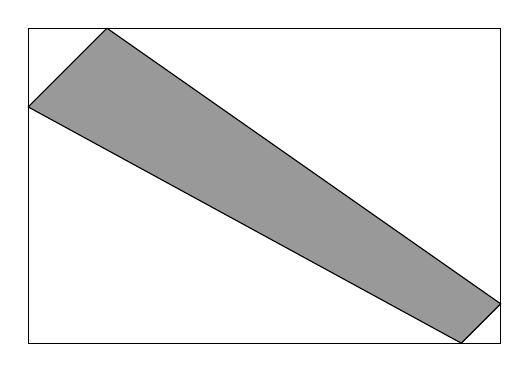
\begin{tikzpicture}[scale=0.5]
                        \draw (0,0) rectangle (12,8);
                        \filldraw[fill=black!40!white, draw=black] (2,8) -- (12,1) -- (11,0) -- (0,6) -- (2,8);
                \end{tikzpicture}
                \caption{Subdirect product}
    \end{subfigure}
    \caption{Direct and subdirect products of the same two intervals $[0,12]$ and $[0,8]$}\label{fig:dirsubdir}
\end{figure}

The subdirect product\footnote{\url{https://en.wikipedia.org/wiki/Subdirect_product}},
standardly defined as a \textit{sub}set of the \textit{direct product} satisfying
projection requirements is not unique: there can be many subsets of the direct
product that project onto both components. This means that the semantics
itself is underdetermined, but this is only to be expected in cases like
noun-noun compounding. Whatever portion of the semantics is rule-governed is
captured, e.g. that in N-N compounding we have `N$_2$ that is V-ed by N$_1$'
with the V indeterminate: ladder \textit{made of} rope, slaughter \textit{undergone
  by} man, tube \textit{used for} test \citep{Kiparsky:1982b}, the
non-compositional part is admitted as suChapter This seems to be the right approach
not just for morphology, but also for the grey zone of \textit{constructions}
between the purely morphological and the purely syntactic such as \textit{NP of
  NP} studied in Berkeley Construction Grammar\footnote{\url{https://www1.icsi.berkeley.edu/~kay/bcg/ConGram.html} \citep{Kornai:1988a}}, taking care of our desideratum
D7.

What are, then, the non-negotiable elements of vector
semantics? One, perhaps the most important one, is the notion of containment,
\textsc{IsA}, which we see as essential for the reconstruction of Aristotelian
\textit{genus}. Whatever definition we provide for \textit{dachshund} or \textit{labrador}, the first thing in the definiens will be \textit{dog}. Given that we
use polytopes (polyhedra-line $n$-dimensional regions) around the word
vectors, \textsc{IsA} comes for free as the set-theoretical inclusion “$\subset$”
relation. This works well for ordinary (intersective) adjectival modifiers
as well: a \textit{brown dog} is in the intersection of the \textit{brown} and the
\textit{dog} polytopes. (For non-intersective adjectives like \textit{former}, see
Chapter 3.2 of \cite{Kornai:2022}).

The method of assigning semantics to \textit{Kim is a donkey} by leveraging
set-theo\-ret\-ical containment cannot be directly generalized.  Clearly,
there is nothing in set theory that would directly work for \textit{Kim has a
  donkey}, but the underlying idea of taking a relation, in this example the
possessive relation \textsc{Has}, and using that for assigning meaning, is
solid. (\textsc{Has} can be further subdivided into inalienable and ordinary
possession, but we will not pursue this matter here.) There remains one
technical difficulty: however the language signals the distinction, \textit{John
  ate the fish} and \textit{The fish ate John} should not be treated as
synonymous. We use \textsc{SubjectOf} and \textsc{ObjectOf} for the
disambiguation. These are good candidates for universality, even in languages
where the distinction is made in absolutive/ergative terms.

With this, we are done -- we don't need further disambiguators (deep cases,
thematic roles or proto-roles, etc.) to get to ditransitive or even higher
arity predicates, since these can be obtained by classic techniques of meaning
decomposition that go back to generative semantics \citep{Kornai:2012}.  (The
\texttt{4lang} system writes \texttt{=agt} and \texttt{=pat}, but we could have
written ``1'' and ``2'' as well -- the only theoretical claim here is that there
is no ``3'' required.) The representation structures we obtain are best depicted
as hypernode graphs that can contain other such graphs as nodes (but not as
edges). These should be familiar from the Resource Description Framework\footnote{\url{https://en.wikipedia.org/wiki/Resource_Description_Framework}} that is standard on the WorldWideWeb.

It is easy to check that the system presented here meets our
desiderata D1 and D8 as well, so our work is done. Readers interested in how the
system can be extended, without adding further operators, to issues of
temporal and spatial semantics, indexicals, negation, quantification,
probability, modality, gradience, implicature, and other issues generally
considered relevant for semantics are advised to look at
\citet{Kornai:2022}. But one word of caution is in order: not having further
operations is not the same as not having further primitives.

The \texttt{4lang} system actually treats a handful of binary relations \textsc{at, between, cause, er, follow, for, from, has, in, ins, isA, lack, mark, on, partOf, under} as primitives (and makes the claim that all others are
derivable). These correspond to matrices, rather than vectors. Remarkably,
what traditional syntax treats as higher order operators, quantifiers in
particular, will require only vectors, rather than full matrices: the central
example is the generic quantifier \texttt{gen}, which simply corresponds to the
$n$-dimensional vector $(1/n,1/n,...,1/n)$ (for details see
\citet{Kornai:2022} Chapter 4.5). The bulk of the primitives are unaries (vectors)
appearing in a system of mutually constraining definitions, and this includes
most verbs that can have an optional object like \textit{eat} as well.

With \textit{eat} it is reasonably easy to see how one can define it in terms of
the Longman Defining Vocabulary `to put food in your mouth and chew and
swallow it' and the process of turning this into a \texttt{4lang} clause can be
automated \citep{Recski:2016d} to yield \texttt{=agt cause\_ \{=pat in mouth\},
  swallow, <=pat[food]>, <bite/1001>, <chew>, =agt has mouth}, which uses an
even smaller defining vocabulary of 739 elements (including the 16 binaries).

Arguably \textit{eat}, if not a universal semantic primitive, is at least very
close to being one, and clearly it is a ``simple'' word \citep{Kornai:2021} that
comes very early in language acquisition. Our earlier example, \textit{awe}, is
clearly far from the simple/basic layer of the vocabulary, but the same method
remains applicable: take the LDOCE definition, in this case `a feeling of
great respect and liking for someone or something', normalize the syntax, and
reduce further until only the \texttt{4lang} primitives remain. We begin with
\textit{for someone or something} and replace it by \texttt{=pat}. \textit{great}
and \textit{liking} are defined, \textit{great} as \texttt{big} and \textit{like} as \texttt{feel \{=pat[good], good for\_ =agt\}}. For \textit{respect}, we have to
go back to LDOCE to obtain ``admire'' , for which we obtain `to look at something
and think how beautiful or impressive it is'. The process goes on, but for
\textit{beautiful} we obtain “extremely attractive” and with \texttt{attract} we
terminate at \texttt{=agt cause\_ \{=pat want \{=pat near =agt\}\}}.

This may appear tedious, but eventually all non-\texttt{4lang} words are
eliminated, since the system was constructed from the Longman Defining
Vocabulary by systematic elimination \citep{Acs:2019b} until a
feedback vertex set\footnote{\url{https://en.wikipedia.org/wiki/Feedback_vertex_set}} is obtained. The price of the termination guarantee is that the resulting set
is considerably larger than the system of Natural Semantic Metalanguage
(NSM; \cite{Wierzbicka:1992,Wierzbicka:1996,Goddard:2002}), which in many ways
served as an inspiration. But \texttt{4lang} both has a formal syntax and
guarantees that all words not defined in the core are definable by it via
LDOCE, whereas NSM uses an informal (English) syntax, and has no guarantees
that words outside the core are actually definable as NSM stanzas.

As for minimality, we make no claim that the set of \texttt{4lang} primitives
is truly minimal, just that by systematic reduction of the entire English
vocabulary we arrived at a stage where we see no further reduction
possibilities.  This does not mean that for other languages no further
reductions would be possible, and it would be an interesting research program
to (i) harden NSM syntax until it becomes machine-parsable and (ii) define the
\texttt{4lang} primitives in terms of the NSM primitives. Whether this is
possible remains to be seen, but our system already provides an upper bound on
the dimension of the vector space we use for modeling semantics.

\section{Conclusions}

Minimality requires thrift both in the number of operations and in the number
of primitives manipulated by these. To maintain compositionality in both
directions, the “bestiary-style” minimalism of (Gödel) numbering has to be
sacrificed for more transparent operations. Of particular interest is the case
when the objects manipulated are vectors and matrices in finite-dimensional
Euclidean space, since these can be acquired gradually, by optimization
techniques that change the vectors only a little bit as new learning data
becomes available, rather than by huge and unpredictable discrete steps that
require a complex system of inborn directives.

As for the primitives, our current system is likely
overcomplete\footnote{\url{https://en.wikipedia.org/wiki/Overcompleteness}}, at least
as far as the vectors (unaries) are concerned, though we seem to approach the
limits of reducibility for the matrices (binary relations) used. Remarkably,
it is not the verbs, transitive, ditransitive, or even higher arity, that
require departure from unary relations, but the prepositions expressing
spatial relations, \textsc{at, between, follow, from, in, on, under,} for which we must
assume a prepositional subject and a prepositional object, the comparative
\textsc{er}, the negative \textsc{lack}, and a few conceptual relation markers,
quite often expressed by cases, such as \textsc{cause, for, has, ins}, and \textsc{partOf}. Pride of place goes to \textsc{isA}, essential for taxonomic
organization, and \textsc{mark}, denoting the relation between the two parts of
the Saussurian sign.

%operate with just \textit{Move} and \textit{Merge}? 





\section*{Acknowledgments} I'm grateful to Geoff Pullum and Bob Levine for
penetrating comments on an earlier draft.

\sloppy
\printbibliography[heading=subbibliography,notkeyword=this]

\end{document}


